\section{Implementierung des SmIdempotencyBackwardRecovery}
Der erste idempotente DEA wird als SmIdempotencyBackwardRecovery bezeichnet. Im Falle eines Netzwerkfehlers bei einem T wird ein Übergang zum entsprechenden C eingeführt; die Saga wird also versucht zurückzurollen, unabhängig ob das T ausgeführt wurde oder nicht. In \cref{fig:fig_sm_idempotency_backward_recovery_testcase2} ist der Fall abgebildet, dass ein T einen Netzwerkfehler verursacht ohne eine Zustandsänderung im Teilnehmerservice zu bewirken. \Cref{fig:fig_sm_idempotency_backward_recovery_testcase3} zeigt den Ablauf im Fall eines Netzwerkfehlers mit Zustandsänderung. 

\begin{figure}[h!]
	\centering
	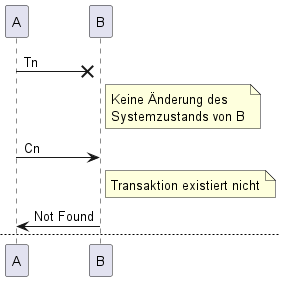
\includegraphics[width=0.3\linewidth]{figures/ChapterVersuchsdurchführung/SmIdempotencyBackwardRecovery-0.png}
	\caption{Sequenzdiagramm für Idempotentes Verhalten bei wiederholten Anfragen in Szenario 3}
	\label{fig:fig_sm_idempotency_backward_recovery_testcase2}
\end{figure}

\FloatBarrier
\begin{figure}[h!]
	\centering
	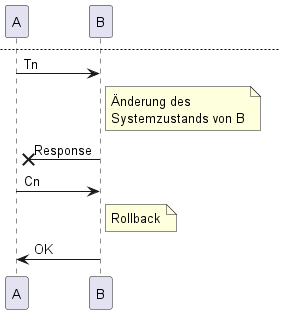
\includegraphics[width=0.3\linewidth]{figures/ChapterVersuchsdurchführung/SmIdempotencyBackwardRecovery-1.png}
	\caption{Sequenzdiagramm für Idempotentes Verhalten bei wiederholten Anfragen in Szenario 3}
	\label{fig:fig_sm_idempotency_backward_recovery_testcase3}
\end{figure}
\FloatBarrier

Solche Fehler treten jedoch auch bei den Cs auf. Deshalb müssen diese auch addressiert werden. Bei Fehlschlagen eines Cs könnte in den Zustand FailedWithoutCompensation gewechselt werden. Dies soll jedoch verhindert werden. Da die Teilnehmerservices idempotentes Verhalten unterstützen, können Cs wiederholt werden, bis ein eindeutiges Ergebnis vorliegt. In folgenden Fällen kann ein Übergang zum nächsten C eingeführt werden:
\begin{itemize}
	\item 200: Die Transaktion wurde erfolgreich kompensiert
	\item 208: Die Transaktion wurde in einem vorherigen Schritt bereits erfolgreich kompensiert
	\item 404: Die Transaktion ist nicht bekannt und muss nicht kompensiert werden
\end{itemize}

Im Falle eines Konflikts (409) muss jedoch weiterhin auf den Zustand FailedWithoutCompensation gewechselt werden.

Der resultierende Zustandsautomat ist in \cref{fig:fig_sm_idempotency_backward_recovery} abgebildet.

\begin{figure}[h!]
	\centering
	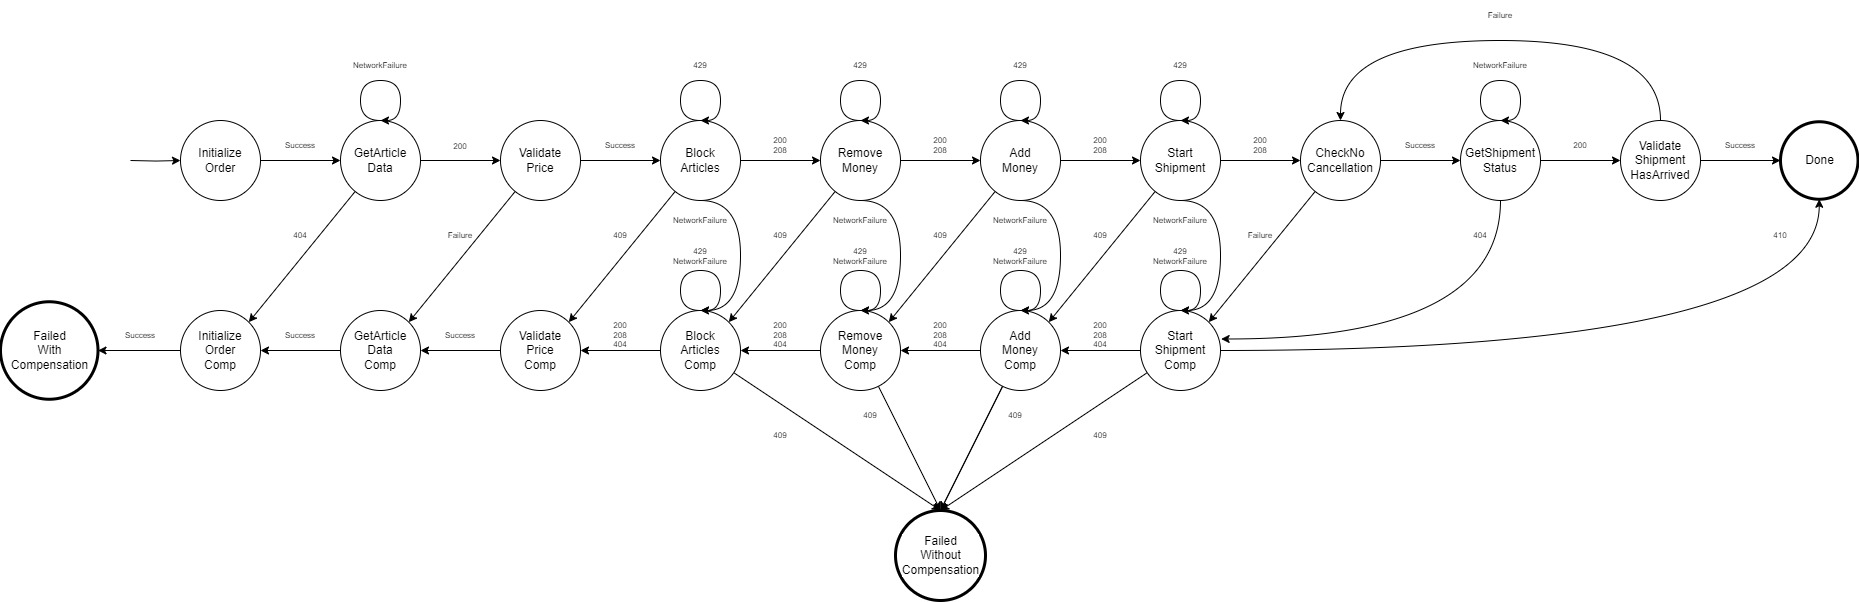
\includegraphics[width=\linewidth]{figures/ChapterVersuchsdurchführung/sm_idempotency_backward_recovery.jpg}
	\caption{DEA für SmIdempotencyBackwardRecovery}
	\label{fig:fig_sm_idempotency_backward_recovery}
\end{figure}
\FloatBarrier

\subsection{StateAnalysisResult}

Das StateAnalysisResult zeigt einen hohen Anteil an vorzeitig abgebrochenen Sagas. Das ist mit dem Konzept der Backwardrecovery begründet. Lediglich Testszenario 1 liefert in beiden Testfällen eine Erfolgsrate von 100\%.

\paragraph*{Testfall FinishOrders}

\begin{center}
	\fontsize{9}{12}\selectfont
	\begin{longtable}[h]{|p{5cm}|p{1cm}|p{1cm}|p{1cm}|}
		\hline
		Messwert & S1 & S2 & S3 \\ \hline
		\endhead
		%\label{tab:smbasic_stateanalysisresult_finishorders}
		\endfoot
		successfull\-Percentage & 1.0 & 0.63 & 0.44 \\ \hline
		finished\-Percentage & 1.0 & 1.0 & 1.0 \\ \hline
		pending\-Percentage & 0.0 & 0.0 & 0.0 \\ \hline
		failedWithCompensation\-Percentage & 0.0 & 0.38 & 0.57 \\ \hline
		failedWithoutCompensation\-Percentage & 0.0 & 0.0 & 0.0 \\ \hline
		hasCorrectEndstate\-Percentage & 1.0 & 0.63 & 0.39 \\ \hline
		containsAllExpectedLogs\-Percentage & 1.0 & 0.63 & 0.44 \\ \hline
		isSuccessfullTestInstance\-Percentage & 1.0 & 0.63 & 0.44 \\ \hline
	\end{longtable}
\end{center}
\FloatBarrier

\paragraph*{Testfall CancelOrders}

\begin{center}
	\fontsize{9}{12}\selectfont
	\begin{longtable}[h]{|p{5cm}|p{1cm}|p{1cm}|p{1cm}|}
		\hline
		Messwert & S1 & S2 & S3 \\ \hline
		\endhead
		%\label{tab:smbasic_stateanalysisresult_finishorders}
		\endfoot
		successfull\-Percentage & 0.0 & 0.0 & 0.0 \\ \hline
		finished\-Percentage & 1.0 & 1.0 & 1.0 \\ \hline
		pending\-Percentage & 0.0 & 0.0 & 0.0 \\ \hline
		failedWithCompensation\-Percentage & 1.0 & 1.0 & 1.0 \\ \hline
		failedWithoutCompensation\-Percentage & 0.0 & 0.0 & 0.0 \\ \hline
		hasCorrectEndstate\-Percentage & 1.0 & 1.0 & 1.0 \\ \hline
		containsAllExpectedLogs\-Percentage & 1.0 & 0.68 & 0.44 \\ \hline
		isSuccessfullTestInstance\-Percentage & 1.0 & 0.68 & 0.44 \\ \hline
	\end{longtable}
\end{center}
\FloatBarrier

\subsection{TransactionAnalysisResult}
In \cref{tab:smbasic_stateanalysisresult} sind die TransactionAnalysisResults für beide Testfälle dargestellt. Überraschend ist hier der niedrige Anteil an konsistenten Sagas in Testszenario 2 und 3. 

\begin{center}
	\fontsize{9}{12}\selectfont
	\begin{longtable}[h]{|p{5cm}|p{1cm}|p{1cm}|p{1cm}|}
		\hline
		& S1 & S2 & S3 \\ \hline
		\endhead
		%\label{tab:smbasic_stateanalysisresult}
		\endfoot
		FinishOrders & 1 & 1 & 0.74\\ \hline	
		CancelOrders & 1 & 1 & 0.74\\ \hline
	\end{longtable}
\end{center}
\FloatBarrier

Die Ursache dafür liegt in der Berechnung der Kennzahl sowie dem Aufbau des Zustandsautomaten. Für die Berechnung der Kennzahl werden die Differenzen der jeweiligen Transaktionen nach Koordinator- und Teilnehmersicht gebildet. Nur wenn diese für jedes T und jedes C übereinstimmen fließt das Ergebnis als erfolgreich in die Kennzahl ein. 

Konkret soll nun diese Messungenauigkeit betrachtet werden. Wird die Anzahl einer Transaktion in Koordinatorsicht berechnet, wird das Transaktionslog verwendet. Dabei soll das in \cref{fig:fig} dargestellte Transaktionslog verwendet werden. 

Das Log zeigt eine Saga, die aufgrund eines Netzwerkfehlers im Zustand \textit{StartShipment} zur Kompensierung wechselt. Zur Berechnung für die Kennzahl \textit{consistentSagasPercentage} wird auch die Anzahl der Transaktionen mit dem Zustand \textit{StartShipment} und dem Ergebnis \textit{StartShipment200} oder \textit{StartShipment208} berechnet. Für den SmIdempotencyBackwardRecovery bedeutet ein Netzwerkfehler in den kritischen Ts, dass das dazugehörige C die Änderungen kompensiert oder fortfährt, falls der Netzwerkfehler keine Zustandsänderungen bewirkt hat. Das Zählen der Transaktionen mit dem Zustand \textit{StartShipment} und dem Ergebnis \textit{StartShipment200} oder \textit{StartShipment208} ist für diesen DEA also keine korrekte Berechnung, um Konsistenz zu messen.

\begin{center}
	\fontsize{9}{12}\selectfont
	\begin{longtable}[h]{|p{4.5cm}|p{6.5cm}|}
		\hline
		Zustand & Ergebnis \\* \hline
		\endhead
		\hline
		\caption{Transaktionslog für Saga im Testfall CancelOrders und Testszenario 2}
		\label{tab:transaktionslog_ts2_cancelorders_smbasic}
		\endfoot
		InitializeOrder & InitializeSagaSuccess \\* \hline
		GetArticleData & GetProductData200 \\* \hline
		ValidatePrice & ValidatePriceSuccess \\* \hline
		BlockArticles & BlockArticles200 \\* \hline
		RemoveMoney & RemoveMoney200 \\* \hline
		AddMoney & AddMoney200 \\* \hline
		\rowcolor{Gray}
		StartShipment & StartShipmentNetworkFailure \\* \hline
		StartShipmentCompensation & StartShipmentCompensationNetworkFailure \\* \hline
		\rowcolor{Gray}
		StartShipmentCompensation & StartShipmentCompensation208 \\* \hline
		AddMoneyCompensation & AddMoneyCompensation200 \\* \hline
		RemoveMoneyCompensation & RemoveMoneyCompensation200 \\* \hline
		BlockArticlesCompensation & BlockArticlesCompensation200 \\* \hline
		ValidatePriceCompensation & ValidatePriceCompensationSuccess \\* \hline
		GetArticleDataCompensation & GetProductDataCompensationSuccess \\* \hline
		InitializeOrderCompensation & InitializeSagaCompensationSuccess \\* \hline
	\end{longtable}
\end{center}
\FloatBarrier

\subsection{Alternative Sicherstellung der Konsistenz}
Damit der Zustandsautomat trotz dieser verfälschten Messung bewertet werden kann, wird eine Alternative benötigt. Um eine Aussage über die Konsistenz zu treffen, kann der Inhalt der eigentlichen Tabellen der Services verwendet werden. 

\paragraph*{Alternative Konsistenzdefinition}\label{par:consistency_definition_alt}
Als Konsistenzkriterien dienen folgende Annahmen:
\begin{itemize}
	\item Die Summe des Geldes im System bleibt gleich.
	\item Die Summer aller Artikel im System bleibt gleich.
\end{itemize}

\paragraph*{Einordnung dieser Definition}
Diese Vorgehensweise kann entscheiden, ob das System nach den definierten Regeln im konsistenten Zustand bleibt oder ob eine Transaktion das System in einen inkonsistenten Zustand überführt hat. Dies ist eine binäre Messung, über die Qualität der Konsistenz kann im vorliegenden System, unter Verwendung dieses Zustandsautomaten und unter Verwendung des aktuellen Versuchsaufbaus keine Aussage getroffen werden. 

Nach den genannten Annahmen ist das System auch konsistent, wenn zwei parallele Sagas fehlschlagen und eine Saga \textit{AddMoney} und die andere Saga \textit{RemoveMoney} jeweils doppelt mit dem (zufällig) identischen Betrag ausführen. Die Menge des Geldes im System bleibt trotz Auftreten eines solchen hypothetischen Bugs konsistent. 

Diese Erläuterung soll verdeutlichen, dass die sehr vage Definition von Konsistenz mit Vorsicht verwendet werden sollte. Für diesen Automaten soll dies jedoch ausreichen. 

\paragraph{Messung}
Die Messung erfolgt manuell. Die Summe des im System befindlichen Geldes wird vor Ausführung der Tests gemessen. Dabei ist jedes Konto mit einem Startcredit von 15000.00 initialisiert. Tritt ein Konsistenzfehler bei Verwendung der BankServices auf, so wird dies in diesem Statement deutlich, wenn sich die zwei Werte \textit{expectedCreditSum} und \textit{actualCreditSum} unterscheiden.

\begin{lstlisting}[language=SQL, breaklines=true, tabsize=2, showstringspaces=false, frame=single, numbers=left, basicstyle=\small] 
select case when 
	15000.00 * cast(
		(select count(*) from bank1user) + 
		(select count(*) from bank2user) as float) 
	= cast(
		(select sum(credit) from bank1credit) + 
		(select sum(credit) from bank2credit) as float)
	then 1 else 0 end as mightBeConsistent;
\end{lstlisting}\label{}

Die Anzahl der Artikel wird mit einem vergleichbaren Statement auf Konsistenz überprüft. Die Summe der Artikel wird über die drei Tabellen des StockServices gezählt. Ändert sich diese Zahl nach Ausführung der Tests, ist ein Konsistenzfehler aufgetreten.

\begin{lstlisting}[language=SQL, breaklines=true, tabsize=2, showstringspaces=false, frame=single, numbers=left, basicstyle=\small] 
select case when 
	(select 15000 * count(*) from articlestock as expectedarticlesum) 
	= 
	(select sum(amount) as amount from (
		select articleid as articleid, amount as amount from articlestock
		union
		select articleid, sum(amount) as amount from blockedarticles group by articleid
		union
		select articleidfk as articleid, sum(amount) as amount from shippedarticles group by articleidfk) as actualarticlesum
	)
	then 1 else 0 end as mightBeConsistent;
\end{lstlisting}\label{}

Ändert sich in beiden Tests die Summe nicht, ist laut \cref{par:consistency_definition_alt} die notwendige Bedingung für Konsistenz erreicht. Das Gesamtergebnis berechnet sich durch folgendes Statement:
\begin{lstlisting}[language=SQL, breaklines=true, tabsize=2, showstringspaces=false, frame=single, numbers=left, basicstyle=\small] 
with moneyMightBeConsistent as (
	select case when 
		(select 15000 * count(*) from articlestock as expectedarticlesum) 
		= 
		(select sum(amount) as amount from (
		select articleid as articleid, amount as amount from articlestock
		union
		select articleid, sum(amount) as amount from blockedarticles group by articleid
		union
		select articleidfk as articleid, sum(amount) as amount from shippedarticles group by articleidfk) as actualarticlesum
	)
	then 1 else 0 end as mightBeConsistent),
articleMightBeConsistent as (
	select case when 
		15000.00 * cast(
			(select count(*) from bank1user) + 
			(select count(*) from bank2user) as float) 
		= cast(
			(select sum(credit) from bank1credit) + 
			(select sum(credit) from bank2credit) as float)
		then 1 else 0 end as mightBeConsistent) 
select moneyMightBeConsistent.mightBeConsistent as moneyMightBeConsistent,
	articleMightBeConsistent.mightBeConsistent as articleMightBeConsistent,
	case when 
		moneyMightBeConsistent.mightBeConsistent 
		= 
		articleMightBeConsistent.mightBeConsistent 
	then 1 else 0 end as mightBeConsistent
from moneyMightBeConsistent, articleMightBeConsistent;
\end{lstlisting}\label{}

\paragraph*{Ergebnis}
Die Messung ist für beide 

\begin{center}
	\fontsize{9}{12}\selectfont
	\begin{longtable}[h]{|p{4cm}|p{1cm}|p{1cm}|p{1cm}|}
		\hline
		 & S1 & S2 & S3 \\ \hline
		\endhead
		\caption{Messwert \textit{altConsistentSagasPercentage} für SmIdempotencyBackwardRecovery}
		\label{tab:smbasic_stateanalysisresult}
		\endfoot
		moneyMightBeConsistent & 1 & 1 & 1 \\ \hline	
		articleMightBeConsistent & 1 & 1 & 1 \\ \hline
		mightBeConsistent & 1 & 1 & 1 \\ \hline
	\end{longtable}
\end{center}
\FloatBarrier
